Priešingai nei daugelis dabartinių vokselius tyrinėjančių autorių darbų, darbe
pristatomu įrankiu stengtasi atskleisti truputį kitą vizualizavimo pusę --
vietoje bandymo pavaizduoti kuo galima dides-nį kiekį vokselių, įrankis
įgalina pavaizduoti gana ribotą kiekį vokselių. Bet masiškumo praradimą jis
kompensuoja vartotojo sąsajos ir parametrų keitimo lankstumu, bei pačio gauto
vaizdo kokybe.

\subsection{Naudota duomenų struktūra}

Šiuolaikinėje realaus laiko grafikai vizualizuoti šiais laikais beveik visada
yra pasitelkiama vaizdo spartintuvų (\emph{Graphics Processing Unit} -- toliau
GPU) pagalba. Neišmintis ir šis darbas. Vienintelis duomenų pasiekimo būdas,
šiuo metu palaikomas GPU, yra tekstūros, į kurias galima žvelgti kaip į
N-mačius masyvus. Šiame darbe pristatomame įrankyje visi tūriniai duomenys yra
saugomi trimatėje tekstūroje, susidedančioje iš RGBA elementų.

\begin{itemize}

\item
\emph{A} komponentė naudojama kaip vokselio permatomumo reikšmė.

\item
\emph{RGB} komponentės naudojamos saugoti gradientą (tarsi „3d normalė“). Gradientas
yra reikalingas apšveitimui.

\end{itemize}

\subsection{Spalvų kubai}

Kaip jau minėta, esminė įrankyje įgyvendinto spindulių sklaidos algoritmo
idėja remiasi spalvų kubais. Tam, kad žinoti, kuriuos trimatės tekstūros
elementus naudoti skaičiuojant fragmento reikš-mę, naudojamas tūrinį objekto
gaubiančio kubo vizualizavimo žingsnis.

Pirma vizualizuojamas tas gaubiantysis kubas, jo lokalias koordinates verčiant
spalvomis (Iliustracija nr. \ref{fig:color_cubes}). Po to vizualizuojamas
gaubiantysis išvirkštinis kubas, koordinates taip pat verčiant spalvomis.

Paprasto kubo spalvos nusako tūrinio objekto pradžios poziciją, o išvirkštinio
-- pabaigos. Abie-jų kubų vizualizacijos perduodamos GPU kaip tekstūros, bet
nėra išvedamos į ekraną.

\begin{figure}[!ht]
\centering
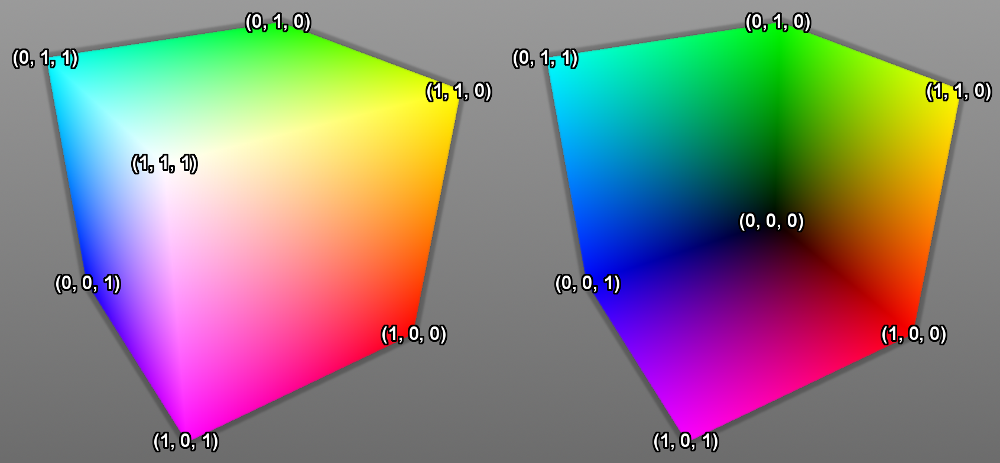
\includegraphics[height=7cm]{color_cubes.png}
\caption{Kairėje pavaizduotas paprastas kubas; dešinėje -- išvirkštinis.}
\label{fig:color_cubes}
\end{figure}

\subsection{Algoritmas}

Pateikiamas algoritmas vienam spindulio skleidimui arba vienam vaizdo gardelės
fragmentui paskaičiuoti. Pristatomame įrankyje šis algoritmas yra vykdomas
darbo autoriaus suprogramuotame GPU fragmentų šeideryje (programa, veikianti
GPU).

\begin{itemize}

\item
Normalaus spalvinio kubo spalvos reikšmė fragmente tampa spindulio kelionės
pradžios taškas

\item
Išvirkštinio spalvinio kubo spalvos reikšmė fragmente tampa spindulio kelionės
pabaigos koordinate

\item
Keliaujame mažu žingsneliu iš pradžios į pabaigos koordinatės poziciją.
Kiekvie-name žingsnelyje kaupiame spalvų ir permatomumo reikšmes pagal šį
ciklą:

\begin{itemize}

\item
Iš duomenų tekstūros nusiskaitome tūrio reikšmę einamoje pozicijoje

\item
Pritaikome transformavimo filtrą

\item
Remdamiesi gradientu, apskaičiuojame apšvietimą

\item
Pritaikome apšveitimo sustiprinimo filtrą

\item
Pritaikome globalų permatomumo filtrą

\end{itemize}

\item
Gautą spindulio skleidimo sankaupos reikšmę išsaugome ir išvedame į ekraną

\end{itemize}

\subsection{GPU panaudojimas}

GPU programuojamumas pasižymi gana dideliais apribojimais. Iš vienos pusės
žvelgiant, tas yra labai nepageidautina. Iš kitos -- tas leidžia GPU
veikiančioms programoms lengvai išskaidyti skaičiavimus į paraleliai
veikiančius GPU procesus.

Pristatomos aplikacijos algoritmas yra būtent toks, koks yra dėl to, kad
norima netrukdyti GPU, kuo galima našiau paskirstyti skaičiavimus. Beveik
visas vizualizacijos generavimas yra paliktas GPU fragmentų procesoriui, nes
pastarasis veiksmas yra izoliuotas nuo aplinkos ir todėl įgalina paskirus
fragmentus apskaičiuoti paraleliai.

Reiktų pabrėžti, kad pačio skaičiavimo išskaidymas nėra įrankio kodo
sudedamoji dalis -- tą atlieka GPU aparatūrinė ir programinė įranga.
Aplikacijoje naudojamas algoritmas tiesiog sudaro sąlygas tam išskaidymui.

\begin{figure}[!ht]
\centering
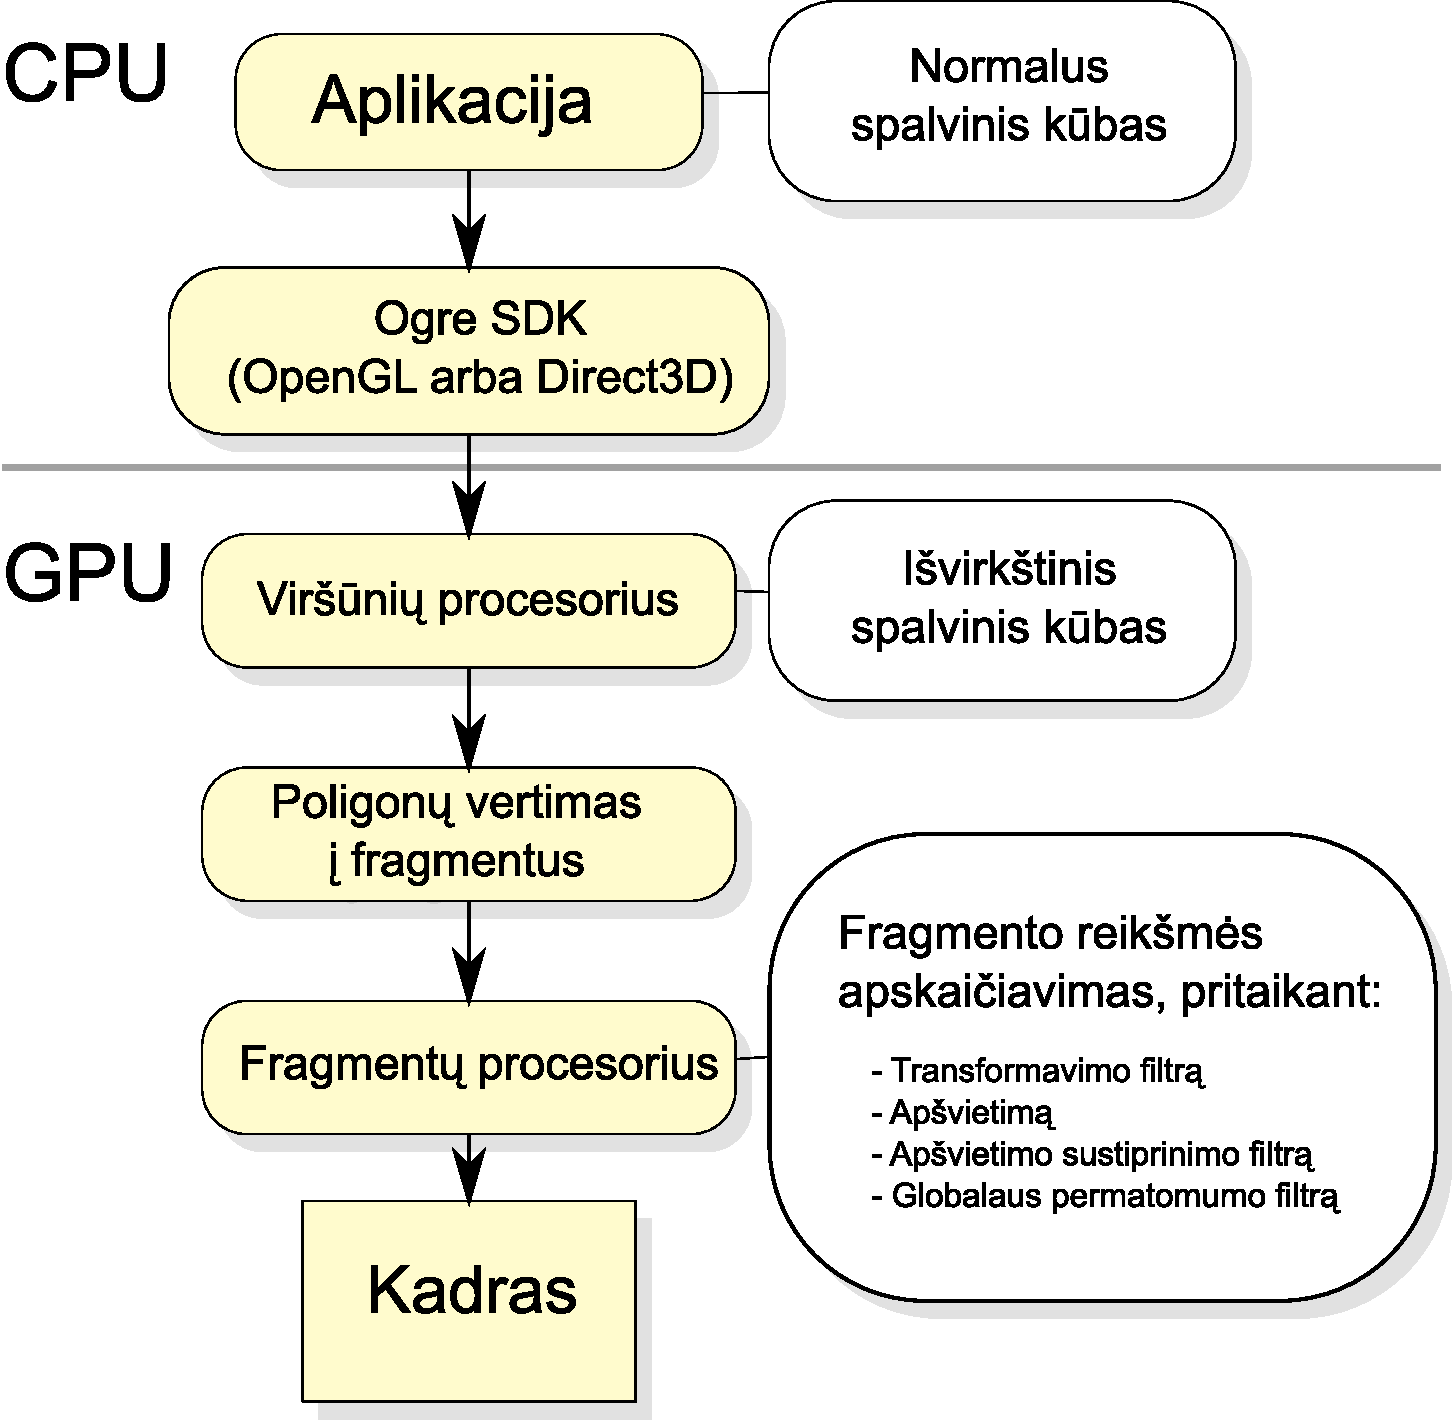
\includegraphics[height=10.0cm]{gpu.pdf}
\caption{GPU panaudojimas įrankyje}
\label{fig:gpu}
\end{figure}

\begin{description}

\item[Aplikacija:] \hfill \\
  Pačioje aplikacijoje apskaičiuojamas normalus spalvinis kubas ir išsaugomas
  tekstūroje, kuri bus nuskaitoma fragmentų procesoriuje. Iš esmės jokio
  skirtumo, kurį kubą pirma skaičiuoti -- galima ir išvirkštinį.

\item[Viršūnių procesorius:] \hfill \\
  Viršūnių procesoriuje apskaičiuojamas išvirkštinis kubas. Tą atlieka
  ganėtinai paprastas skriptas, kuris didžiąją dalį darbo palieka GPU
  aparatūrinei įrangai ir GPU tvarkyklėms.

\item[Fragmentų procesorius:] \hfill \\
  Fragmentų procesoriuje atliekami visi pagrindiniai skaičiavimai, kombinuojant
  abiejų spalvinių kubų ir 3D tekstūroje saugomų vokselių duomenų reikšmes.

\end{description}


\subsection{Transformavimo filtras}

Transformavimo filtras yra funkcija, kurios argumentas yra permatomumo
reikšmė, o rezultatas yra spalva ir nauja permatomumo reikšmė.

$$
F(a') \to \vec{(r, g, b, a)}
$$

\begin{figure}[!ht]
\centering

\includegraphics[height=2.0cm]{transfer.png}
\caption{Permatomumo skalė $0.0 \ldots 1.0$ transformuojama į naują
permatomumo reikšmę, tuo pačiu pridedant spalvos komponentes.}
\label{fig:transfer}
\end{figure}

Transformavimo filtras (Kartais dar vadinamas transformavimo funkcija) buvo
pasiūlytas dar 1988 m., Robert A. Drebin ir kitų veikale \emph{„Volume
Rendering“} \cite{transfer}. Tiesa, tuo metu jie naudojo terminą
klasifikatorius -- „transformavimo funkcija“ terminas buvo pradėtas naudoti
žymiai vėliau. Mano įvesta naujovė yra ta, kad įrankyje transformavimo filtrą
galima keisti realiu laiku. Pokyčiai vizualizacijose vyksta taip pat
realiame laike.

\subsection{Apšvietimo sustiprinimo filtras}

Vizualizuojant tūrinius objektus, turinčius (ar transformavimo funkcijos dėka,
įgaunančius) mažas permatomumo reikšmes, buvo pastebėta, kad detalės pernelyg
susilieja. Tam spręsti siūlomas apšvietimo sustiprinimo filtras.

$$
F(r, g, b, a) = X \cdot D(r, g, b, a) + A(r, g, b, a) + E(r, g, b, a) \to \vec{(r, g, b, a)}
$$

Kur $X$ yra šio filtro parametras; $D$ apšvietimo sklaidos (\emph{diffuse});
$A$ -- apsupties (\emph{ambient}); $E$ -- aplinkos (\emph{environment})
apšvietimo reikšmes skaičiuojančios funkcijos. Pastaba: gradientai, pozicijos
(kameros, šviesos šaltinio, vokselio) aiškumo dėliai yra išmesti iš formulių.

Sustiprinant/susilpninant apšvietimo sklaidos komponentės reikšmę $X$ netgi
iki bendrai 3D apšvietimo logikai prieštaraujančių reikšmių, išryškėja kai
kuri dalis „pasislėpusių“ tūrinio objekto detalių.

\subsection{Globalus permatomumo filtras}

Globalus permatomumo filtras, tai taip pat kuriant įrankį sugalvotas ir šiame
veikale pasiūlytas filtras, kuris savyje kombinuoja tiek slenksčio, tiek
permatomumo reikšmės sustiprinimo/susilpni-nimo filtrus.

$$
F(r, g, b, a) =
\left\{
  \begin{array}{ll}
  (r, g, b, a \cdot X) & \mbox{jeigu $a > X$}\\
  (0, 0, 0, 0) & \mbox{jeigu $a \leq X$}
  \end{array}
\right. \to \vec{(r, g, b, a)}
$$

Kur $X$ yra šio filtro parametras. Pačioje pradžioje, kuriant įrankį, buvo
naudojamas paprastas slenksčio filtras. Tačiau sugeneruotas vaizdas pasižymėjo
grubiais „peršokimais“ slenksčio ribose. Norint to išvengti buvo sugalvotas
filtras, kurio esmė yra siūlymas permatomumą riboti ir slenksčio prieigose.

\subsection{Vokselių trynimo funkcija}

Realaus laiko kompiuterinė grafika skiriasi nuo prieš rodymą sugeneruotos
dviem dalykais: interaktyvia navigacija ir virtualaus pasaulio keitimu.

Pristatomame įrankyje navigacija yra neribojame -- galima judėjimas bet kuria
kryptimi ir kame-ros sukiojimas leidžiamas bet kokiu kampu.

Nenorint palikti virtualaus pasaulio (aprašomos aplikacijos atveju tiesiog
įrankyje rodomo tūri-nio objekto) keitimo funkcijos nuošalyje, yra įdiegtas
grynai demonstracinio pobūdžio vokselių trynimo funkcionalumas.

Tai labai paprastą funkcionalumą turintis įrankio modulis. Jis įgalina
vartotoją šaudyti kiaurai tūrinį objektą. Atlikus šį veiksmą, šūvio kelio
aplinkoje yra pašalinami vokseliai, atliekant aibių skirtumo operaciją.
(Pav. \ref{fig:delete_voxels1} ir \ref{fig:delete_voxels2}).

Šio redagavimo funkcionalumo esmė yra parodyti, kad įrankyje rodomas iš
vokselių sudarytas tūrinis objektas yra vizualizuojamas realiu laiku,
nepritaikant jokių optinių apgaulių ir nesinaudojant jokiais podėliais.
„Šaunant“ per tūrinį objektą, vartotojui iškart yra pateikiamas nauja,
pakitusi vokslelių vizualizacija.

\begin{figure}[t]
\centering
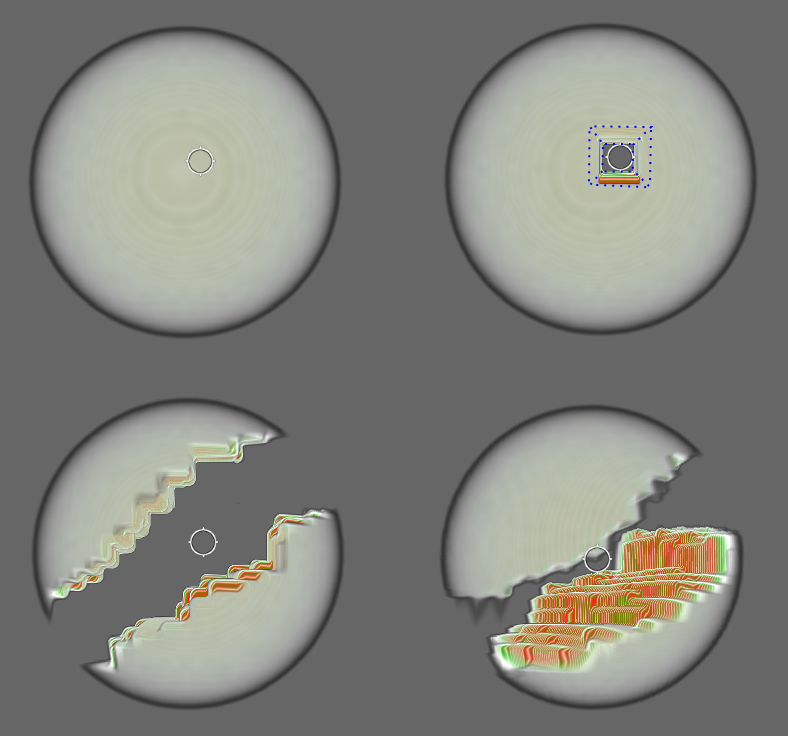
\includegraphics[height=8cm]{delete1.png}
\caption{Vokselių trynimas.}
\label{fig:delete_voxels1}
\end{figure}

\begin{figure}[t]
\centering
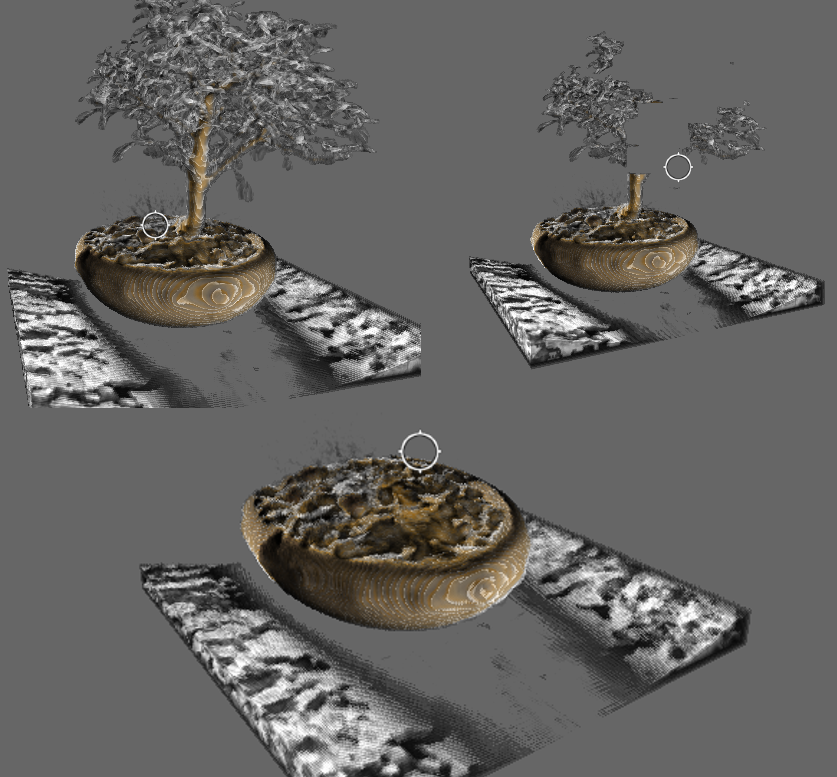
\includegraphics[height=8cm]{delete2.png}
\caption{Vokselių trynimas.}
\label{fig:delete_voxels2}
\end{figure}


\subsection{Naudotos technologijos}

Įrankis kurtas naudojantis šiomis technologijomis: C++ programavimo kalba, Qt
vartotojo sąsajos bibliotekas, OGRE grafinį varikliuką ir Cg šeiderių rašymo
programavimo kalbą.

\subsubsection{OGRE}

OGRE (Object-Oriented Graphics Rendering Engine) yra atviro kodo, lankstus
trimatės kompiuterinės grafikos variklis, sukurtas su C++ programavimo kalba.

Pagrindiniai jo privalumai:

\begin{itemize}

\item
  Atviras kodas

\item
  Palaikoma daugumoje Operacinių sistemų (MS Windows, Linux, Mac OS).

\item
  Palaiko tiek OpenGL ir Direct3D. OGRE variklis leidžia nekreipti dėmesio į
  tai, su kokiomis grafinėmis tvarkyklėmis veikia juo parašyta aplikacija.
  Multiplatformiškumas tampa dvigubas: tiek OS, tiek grafinių tvarkyklių
  požiūriais.

\item
  Lankstumas. Šis variklis netrukdo, jeigu bandoma atlikti kažką egzotiško
  ir/ar neįprasto.

\item
  Bibliotekos moduliai suteikia patogų funkcionalumą daugeliui standartinių
  veik-smų -- susitaupo daug laiko, nes nereikia rašyti pasikartojančio,
  trivialaus kodo.

\end{itemize}

\subsubsection{Qt}

Qt yra multiplatforminis aplikacijų ir vartojo sąsajos kūrimo bibliotekų
rinkinys. Biblioteka skirta grafiniai vartotojo sąsajai sukurti. Ji buvo
naudota langams, bei dialogams sukurti, įvesties (pelė, klaviatūra) veiksmas
apdoroti. Qt pasirinkimą lėmė šios savybės:

\begin{itemize}

\item
  Multiplatforminė biblioteka. Jeigu būtų pasirinkta ne multiplatforminė --
  būtų prarasta visa nauda, gaunama iš to, kad OGRE yra multiplatforminė.

\item
  Atviras kodas.

\item
  Puiki dokumentacija.

\item
  Lengva integracija su OGRE.

\end{itemize}

\subsubsection{Cg}

Cg -- NVidia kompanijos sukurta programavimo kalba, skirta aprašyti GPU
programuojamuo-se procesoriuose vykdomas komandas (\emph{shaders}) (tiek
fragmentų, tiek viršūnių, tiek geometrijos). Išskirtinė tuo, kad kitaip nei
GLSL ar HLSL programavimo kalbos, šioji gali būti kompiliuojama tiek į GLSL,
tiek į HLSL, tiek į asemblerinį išeities kodą. Kaip jau minėta, OGRE įgalina
paleisti pristatomą įrankį tiek OpenGL, tiek Direct3D tvarkykles naudojančiose
OS. Cg pasirinkimas leidžia išlaikyti šį multiplatformiškumą.

\subsection{Apšvietimas}

Vaizdas tėra formos ir apšvietimas. Paprastai kompiuterinėje grafikoje
apšvietimas skaičiuojamas, pasitelkiant paviršių normalias, susietas su
poligonų viršūnėmis. Tuo tarpu įrankyje nėra vizualiai matomų poligonų -- yra
tik vokseliai.

Apšviestiems tūriniams objektams vizualizuoti yra naudojamas gana standartinis
metodas -- kiekvienam vokseliui yra paskaičiuojamas jo permatomumo gradientas.
Įgyvendinant gradientų skaičiavimą buvo remtasi Harvey Ray ir kitų
\cite{gradients} pateiktu apytiksliu gradientų skaičiavimo metodu. Tas
gradientas yra naudojamas kaip normalė standartinėje kompiuterinės grafikos
apšvietimo schemos realizacijoje.

Apytikslio vokselio gradiento, esančio pozicijoje $(i, j, k)$, skaičiavimo
formulė:

$$
G =\Big( \frac{S_{i+1, j, k} - S_{i-1, j, k}}{\Delta x} ,
         \frac{S_{i, j+1, k} - S_{i, j-1, k}}{\Delta y} ,
         \frac{S_{i, j, k+1} - S_{i, j, k-1}}{\Delta z})
$$

Kur $S_{i', j', z'}$ yra vokselio permatomumo (ar tankumo) reikšmė pozicijoje
$(i', j', z')$, o $\Delta a$ -- vokselių atstumas koordinatės $a$ atžvilgiu.

Kadangi toks gradientų skaičiavimas nėra visiškai tikslus, tai ganėtinai mažą
vokselių kiekį turinčių objektų vizualizacijos turi nepageidaujamus
artefaktus. Ši problema įrankyje buvo išspręsta, paliekant galimybę išjungti
apšvietimą. Net ir išjungus apšvietimą, įrankis objektus vizualizuoja
atsižvelgdamas į vokselių nutolimą nuo kameros. Taip vaizdui yra suteikiamas
gilumo pojūtis (Pav. \ref{fig:lighting}).

\begin{figure}
\centering
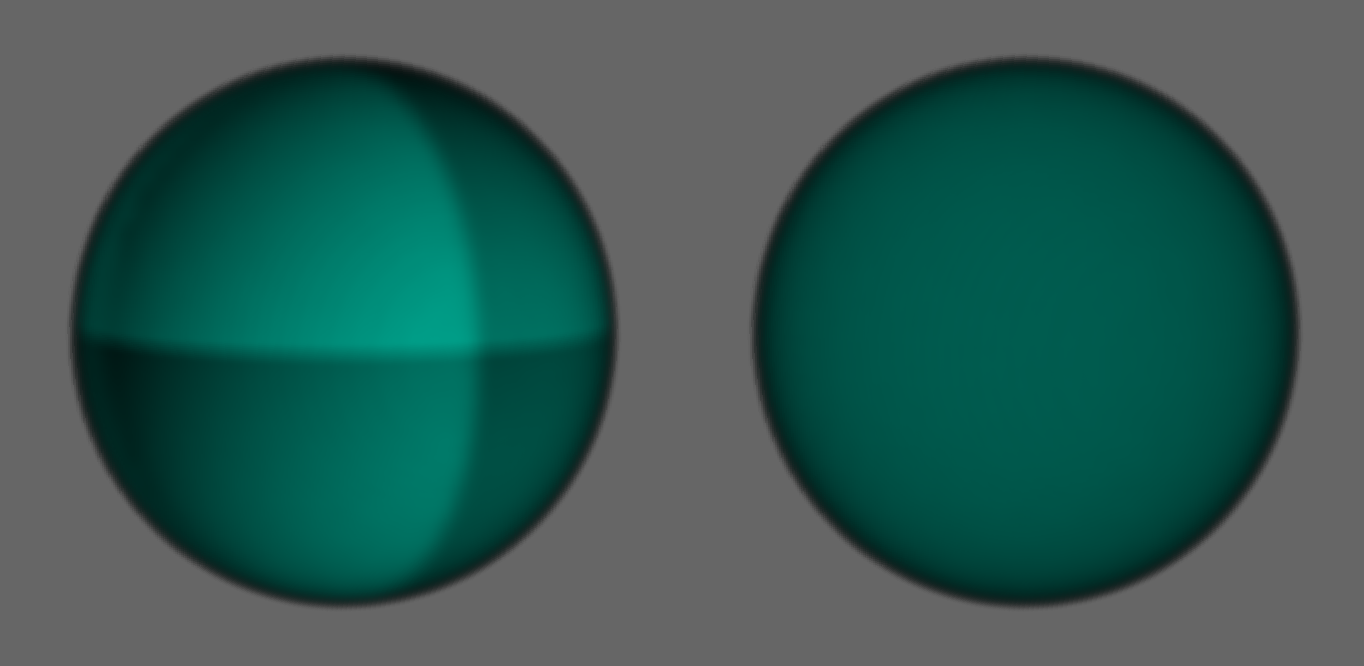
\includegraphics[height=6.0cm]{lighting.png}
\caption{Su apšveitimu ir apšvietimo artefaktais (kairėje); Be apšvietimo
(dešinėje). Pastaba: šviesos šaltinio ir kameros pozicijos specialiai
pasirinktos taip, kad išgauti kuo prastesnį vaizdą.}
\label{fig:lighting}
\end{figure}

\subsection{Spalvoti multi kubai}

Susijusių darbų (\ref{sec:susije_darbai} skyrius) apžvalgoje buvo minėta, kad
daugelis autorių šiuo metu stengiasi pavaizduoti kuo didesnį kiekį vokselių.
Norėdami tą atlikti realiu laiku, jie daro tam tikras prielai-das ir
apribojimus. Tokius kaip:

\begin{itemize}

\item
  Erdvė daugiausia susideda iš tuštumos arba nepermatomų objektų.

\item
  Įvairiose aplikacijose (Pavyzdžiui žaidimuose) vartotojas mato tik nedidelę
  sce-nos dalį.

\item
  Dalinai permatomi objektai retai kada pasitaiko ir dažniausiai yra
  susispietę tam tikrose scenos vietose.

\end{itemize}

Tokios ir panašios prielaidos leidžia jiems atlikti daug optimizacijų.  Tuo
tarpu čia pristatomo įrankio kūrėjas negalėjo sau leisti panašių prielaidų.
Visų pirma dėl to, kad būdama vizualizavimo ir {\bf normavimo} įrankiu,
aplikacija privalo galėti rodyti visą sceną vienu metu. Visų antra, dėl to,
kad yra įgyvendintas interaktyvus transformavimo filtro keitimas, įrankis
negali žinoti, kokias permatomumo reikšmes vokseliai įgis kito kadro metu -- o
reikšmės gali keistis kardinaliai.

Taigi, įrankis priverstas visą sceną laikyti GPU operatyvioje atmintyje.
Norint šiek tiek padidinti kadrų per sekundę skaičių, buvo sugalvota spalvotų
kubų idėją šiek tiek pakoreguoti ir buvo sugalvota spalvotų multi kubų idėją.
Užbėgant už akių, deja, reikia pripažinti, kad pastaroji idėja nedavė jokių
teigiamų rezultatų.

Spalvotų multi kubų idėja ganėtinai paprasta -- vietoje vienos didelės 3D
tekstūros, saugoti scenos tūriniams duomenims, vokseliai yra saugomi $NxNxN$
3D tekstūrose. Buvo tikimasi, kad dėl procesorių gausos GPU, daug mažų
tekstūrų bus našesnis sprendimas, nei viena didelė. Vizualizuojant, buvo
generuojamas vienas išvirkštinis ir $NxNxN$ normalūs spalviniai kubai (Pav.
\ref{fig:multi_color_cubes}).

\begin{figure}[!ht]
\centering
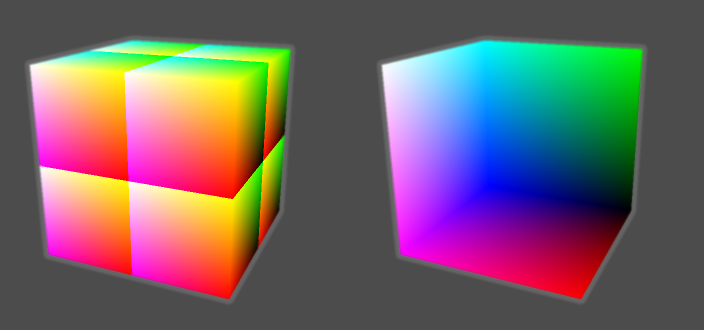
\includegraphics[height=6cm]{multi_color_cubes.png}
\caption{Spalvotų multi kubų idėja}
\label{fig:multi_color_cubes}
\end{figure}

Rezultatai (Lentelė \ref{tab:multi_color_cubes}) nerodo jokių teigiamų pokyčių
\footnote[1]{Naudota techninė įranga: Intel Pentium(R) 4 CPU 3.00GHz; 1 GB
RAM; NVIDIA GeForce 9500 GT (512 MB Ram). Vaizdavimo rezoliucija $846x464$.}
:

\begin{table}[!ht]
\centering
  \begin{tabular}{ | r | r | r | r | }
  \cline{2-4}
  \multicolumn{1}{c|}{} & \multicolumn{3}{|c|}{Scenos padalijimas} \\ \cline{2-4}
  \multicolumn{1}{c|}{} & $1x1x1$ & $2x2x2$ & $4x4x4$ \\ \hline
  262144 vokseliai      &  101.42 &   98.05 &   77.26 \\ \hline
  16777216 vokseliai    &   65.51 &   65.25 &   59.09 \\ \hline
  \end{tabular}
\caption{Spalvotų multi kubų įtaka kadrų per sekundę skaičiui}
\label{tab:multi_color_cubes}
\end{table}

Paaiškėjo, kad (bent jau su testuota aparatūrine įranga) pats suskaidymas neduoda
jokios ap-čiuopiamos naudos -- tiesiog prarandami keli kadrai per sekundę dėl
papildomo darbo skaičiuojant multi kubus.

Tiesa, yra vienas tokio suskaidymo privalumas. Naudojant ją yra įmanoma
pavaizduoti net ir tokias scenas, kurios dėl vokselių skaičiaus netelpa į GPU
atmintį -- ko nebuvo galima atlikti be jos. Reikia pastebėti, kad netelpant
scenai į atmintį, kadrų per sekundę skaičius būna nukritęs į tokias žemumas,
jog to nebegalima vadinti „realiu laiku“.

Taip pat yra dar vienas galimas privalumas. Tikėtina, kad toks ar panašus
priėjimas prie vokselių vizualizavimo duotų naudos, naudojant ne vieną, o
kelis GPU vienu metu. Tačiau tyrimai šia kryptimi nebuvo atlikti dėl to
paprastos priežasties -- autorius neturėjo prieigos prie tokią komplektaciją
turinčios aparatūrinės įrangos.

